%latex->pdf
\documentclass[11pt]{article}
\usepackage{amssymb}
\usepackage{amsmath}
\usepackage{a4wide}
\usepackage[dutch]{babel}
\usepackage{pstricks}
%\usepackage{pst-pdf}
\usepackage{wrapfig}
\usepackage{graphicx}
\parindent=0mm

\newcommand{\andspaceNL}{\hspace{10mm} {\rm en} \hspace{10mm}}
\newcommand{\RR}{\ensuremath{\mathbb{R}}}
\newcommand{\ZZ}{\ensuremath{\mathbb{Z}}}
\newcommand{\QQ}{\ensuremath{\mathbb{Q}}}
\newcommand{\NN}{\ensuremath{\mathbb{N}}}
\newcommand{\CC}{\ensuremath{\mathbb{C}}}
\newcommand{\rarr}{\rightarrow}
\newcommand{\ds}{\displaystyle}
\newcommand{\Rnulplus}{\ensuremath{\mathbb{R}_0^+}}
\begin{document}

{\Huge\textbf{Voorkennisles 2}}

 \section{Inverse functies}

\subsection*{Voorbeeld 1}
Stel $f$ de functie met voorschrift $f(x) =  x^3$, of anders
genoteerd: $y = x^3$. 
\begin{itemize}
\item We zeggen dat $y$ een functie is van $x$ want bij
elke $x$ hoort er een unieke $y$, namelijk $x^3$. Bijvoorbeeld als $x=2$, dan is $y = 2^3 = 8$
\item Is $x$ ook een functie van $y$? Als $y = f(x) = 8$, wat is dan $x$? De
vergelijking $x^3 = 8$ heeft als UNIEKE oplossing $x = 8
^\frac{1}{3} = 2$.
\end{itemize}

In dit voorbeeld geldt dat voor elke $y$ er een UNIEKE $x$ is zodat
$x^3 = y \Leftrightarrow x = y^\frac{1}{3}$. We kunnen dus
zeggen dat $x$ een functie is van $y$, bij elke $y$ hoort er immers
een unieke $x$ namelijk $y^\frac{1}{3}$.

 Daarom noemen we de
functie $g$ met als voorschrift $g(y) = y^\frac{1}{3}$ de inverse
functie van $f$. De inverse functie van $f$ wordt ook genoteerd met
$f^{-1}$, dus $f^{-1} (y) = y^\frac{1}{3}$. We hoeven voor de
inverse functie niet de letter $y$ te gebruiken als variabele, we
kunnen ook noteren: $f^{-1}(x) = x^\frac{1}{3}$. Merk ook op dat:
\begin{itemize}
\item $f\left(f^{-1}(x)\right)= f (x^\frac{1}{3}) = (x^\frac{1}{3})^3 = x$
\item $f^{-1}\left(f(x)\right)= f^{-1}(x^3) = (x^3)^\frac{1}{3} =x$
\end{itemize}
\subsection*{Algemeen:}

\label{inverse functie}
\begin{itemize}
%\item $y = f(x) \Longleftrightarrow x = f^{-1}(y)$
\item $f\left(f^{-1}(x)\right)=x$
\item $f^{-1}\left(f(x)\right)=x$
\end{itemize}
\subsection*{Voorbeeld 2}
Stel $f$ de functie met voorschrift $f(x) =  x^2$, of anders
genoteerd: $y = x^2$.
\begin{itemize}
\item als $x=2$ dan is $y = 2^2 = 4$
\item als $f(x) = 4$, wat is dan $x$? De
vergelijking $x^2 = 4$ heeft GEEN UNIEKE oplossing, zowel $x = 4
^\frac{1}{2} = 2$ en $x = - 4 ^\frac{1}{2} = - 2$ zijn oplossingen.
\end{itemize}
Om toch een inverse te kunnen nemen van $f$ moeten we het domein van
$f$ beperken tot bijvoorbeeld de positieve getallen. De functie
$f_1(x) = x^2$ met $x \geq 0$ heeft wel een inverse functie,
namelijk $f_1^{-1}(y) = \sqrt y $ met $y \geq 0$.

\section{Exponenti\"{e}le en logaritmische functies}
\subsection*{Inleiding}
Schets de grafiek van $f(x) = 2^x$:

\vspace{5cm}

Schets de inverse functie van $f(x) = 2^x$, deze noteren we met
$f^{-1}(x) = \log_2(x)$:

\vspace{5cm}

Voor inverse functies geldt $y = f(x) \Leftrightarrow x = f^{-1}(y)
$, dus $ y = 2^x  \Leftrightarrow x = \log_2(y) $.

\subsection*{Definitie (cursus p 63)}
Voor $a>0$ en $a \neq 1$ : $y = a^x  \Leftrightarrow  x = \log_a y $     \\
 $\log_a y = $ macht waarmee
je $a$ moet verheffen om $y$ te krijgen.

\subsection*{Eigenschappen (niet in cursus)}
$$\displaystyle a^{\log_a x} = x$$
$$\log_a a^y = y$$
voorbeeld: $\log_2 8 = \log_2 2^3 = 3$
\subsection*{Speciale gevallen}
\begin{itemize}
\item $a=10$ \hspace{1cm} $\log_a x = \log x$
\item $a=e$ \hspace{1cm} $\log_a x = \ln x$
\end{itemize}
\newpage
 Geef de grafiek van $f(x)=e^x$ en $f(x)=\ln x$, de definitie en de
eigenschappen van ln: \vspace{4.3cm}


\subsection*{Rekenregels}
\label{rekenregels_log}
$x>0, x_1>0,x_2>0$

\begin{enumerate}

\item
%De logaritme van een product is de som van de logaritmen.
$  \log_a\ (x_1 x_2)\ =\  \log_a x_1\ +\  \log_a x_2 $
\item
%De logaritme van een quoti\"{e}nt is het verschil van de logaritmen.\\
$  \log_a \frac{x_1}{x_2}\ =\  \log_a x_1\ -\  \log_a x_2 $
\item
%De logaritme van een macht is gelijk aan een veelvoud van de logaritme. \\
$  \log_a (x^{r})\ =\ r \  \log_a x$
\item Overgang van logaritme naar logaritme met een ander grondtal:
$\displaystyle  \log_b x\ =\ \frac{ \log_a x}{\log_a b} $
\begin{itemize}
\item vb1: neem $b=10$ en $a=e$:
\vspace{2mm}
\item vb2: neem $x=a$:
\end{itemize}
We kunnen rekenregel 4. ook schrijven als:
\end{enumerate}
\subsection*{Oefeningen}
 \begin{enumerate}

 \item Los volgende vergelijkingen op:
\begin{enumerate}
\item $5^x = 7$
\item $\ln(x^3) = -1$
\end{enumerate}

\item Bereken zonder rekenmachine.
\label{oeflog}
\begin{enumerate}
%\item $\log_2 64$
\item $\log_5 125$
\item $\ds{\log_2 \frac{1}{32}}$
\item $\log_6 (36 \sqrt{6})$
\item $\ds{\log 0,00001}$
\item $\ds{\log_4 \left(\log_4 (4^{\frac14})\right)}$
\end{enumerate}



\item Schrijf als combinatie van $\log a$, $\log b$ en $\log
c$ ($a,b,c>0$).  Vb: $\ds{\log \frac{a}{b^4}} =  \log a - 4 \log b$
 \label{oeflogalogb}
\begin{enumerate}
\item $\ds{\log \left( c^3 \sqrt{\frac{a}{b}} \right)}$
\item $\ds{\log \frac{a^4 b c}{\sqrt{bc^2}}}$
\end{enumerate}

\item  De vergelijking $\ds{4^x-5\cdot2^x=24}$ werd opgelost naar $x$. Toch klopt de oplossing niet
als we deze terug invullen in de vergelijking. Zoek de fout in de
redenering en geef de juiste oplossing. \label{oef:logzoekfout}
\begin{align*}
2^{2x}-5\cdot2^x=&\ 24\\
\log_22^{2x}-\log_2(5\cdot2^x)=&\ \log_224\\
2x-\log_25-\log_22^x=&\ \log_224\\
2x-\log_25-x=&\ \log_224\\
x=&\ \log_224+\log_25\\
x=&\ \log_2 (24\cdot5)\\
x=&\ \log_2120\\
\end{align*}

%\item Schrijf elke uitdrukking als combinatie van $\log x$, $\log(x-5)$ en $\log(x+1)$.
%\label{oeflogx}
%\begin{enumerate}
%\item $\ds{\log\frac{x(x+1)}{x-5}}$
%\item $\ds{\log\left((x+1)^2\sqrt{x-5}\right)}$
%\item $\ds{\log\sqrt{\frac{x-5}{x^3(x+1)}}}$
%\item $\ds{\log\frac{1}{(x+1)^2}}$
%\end{enumerate}

\item Schrijf elke uitdrukking als \'e\'en enkele logaritme.
\label{oef��nlog}
\begin{enumerate}
\item $\ds{\log(x+1)-\log x^2+\frac{1}{2}\log(x-3)}$
\item $\ds{3-\log x}$
\item $\ds{5\log(x-1)-\frac{1}{2}\log(x+3)}$
\end{enumerate}

\item Schrijf onderstaande uitdrukking als combinatie van $\log(k-1)$, $\log k$ en $\log(k+1)$.
\label{oeflogk}
\[\log\left(1-\frac{1}{k^2}\right)\]

\item Toon aan dat:
\label{oefchemie1}
\begin{enumerate}
\item $\ds{\log \frac{a}{b} - \log \frac{c}{d} = - \log \frac{b}{d} +
\log \frac{a}{c}}$
\item $\ds{ - \log \frac{1}{a} + \log \frac{1}{b} = - \log
\frac{b}{a}}$
\end{enumerate}
opmerking: de rekenregels gebruiken zoals in deze oefening, moet
je ook vlot kunnen wanneer hier grootheden uit de chemie of fysica
staan in plaats van a, b, c en d.

\item Enkele oefeningen uit de chemie. Je hoeft de betekenis van
de gebruikte symbolen niet te kennen om de oefening te kunnen
oplossen (niet voor Informatica). \label{oefchemie2}
\begin{enumerate}
\item Gegeven $\ds{ \Delta G^0 =  - n. F.  \Delta E^0}$ en $\ds{\Delta G^0 =  -R.
T.\ln(K_{ev})}$. \\\\Toon aan dat $\ds{K_{ev} =  10^{\ds \frac{n.
F. \Delta E^0}{2,303. R .T}}}$.
\item Gegeven $0,89 = 1,5 - \ds \frac{0,059}{2} \log_{10}
\ds \frac{1}{\frac{10^{-14}}{K_a} 10^{-14}}$. \\\\Toon aan dat
$K_a = 4,7. 10^{-8}$.
\end{enumerate}

\item
\label{oefchemie3}
Schets de grafiek van de functie $\ln C(t)$ met
$C(t) = 3 e^{-2 t}$.
%\item Schets de grafiek van $\ln k$ in functie van $\ds \frac{1}{T}$
%met $k = A e^{-\ds \frac{E}{R T}}$.




\item Onderzoek welke $x\in \RR$ voldoen aan
 \begin{enumerate}
\item $ \displaystyle e^{\ds \sqrt{x}\ln(1/2)}< e^{\ds
5\ln(1/2)}$
\item $ \displaystyle \ln( ( \frac{1}{\sqrt x} + \frac67)^3) > 0$
\end{enumerate}


\end{enumerate}
\subsection*{Enkele oplossingen}
\begin{enumerate}
\item[1.]
\begin{enumerate}
\item $x = \log_5 7$
\item $x = e^{- \frac13}$
\end{enumerate}
\item[2.]
(a) 3, (b) -5, (c) $\frac{5}{2}$, (d) -5, (e) -1

\item[3.]
\begin{enumerate}
\item $ 3 \log c + \frac{1}{2} \log a - \frac{1}{2} \log b$
\item $4 \log a + \frac{1}{2} \log b$
\end{enumerate}
\item[4.] $x=3$
%\item[5.]
%\begin{enumerate}
%\item $\log x + \log (x+1) - \log (x-5)$
%\item $2 \log(x+1) + \frac{1}{2} \log (x-5)$
%\item $\frac{1}{2} \log(x-5) -\frac{3}{2} \log x - \frac{1}{2} \log
%(x+1)$
%\item $-2\log (x+1)$
%\end{enumerate}
\item[6.]
\begin{enumerate}
\item $\log \ds\frac{(x+1)(x-3)^\frac{1}{2}}{x^2}$
\item $\log \ds \frac{10^3}{x}$
\item $\log \ds\frac{(x-1)^5}{(x+3)^\frac{1}{2}}$
\end{enumerate}
\item[7.] $\log (k-1) + \log (k+1) -2 \log k$

%\item[10.] Dit is een rechte. Duid het snijpunt met de verticale
%as en de richtings\-co\"{e}ffici\"{e}nt aan.
\item[11.] \begin{enumerate}
\item $]25, +\infty[$
\item $]0,49[$
\end{enumerate}

\end{enumerate}
\section {Limieten}
%\subsection*{De functie $f(x) = \frac{1}{x}$}
%\begin{center}
%\scalebox{0.2}{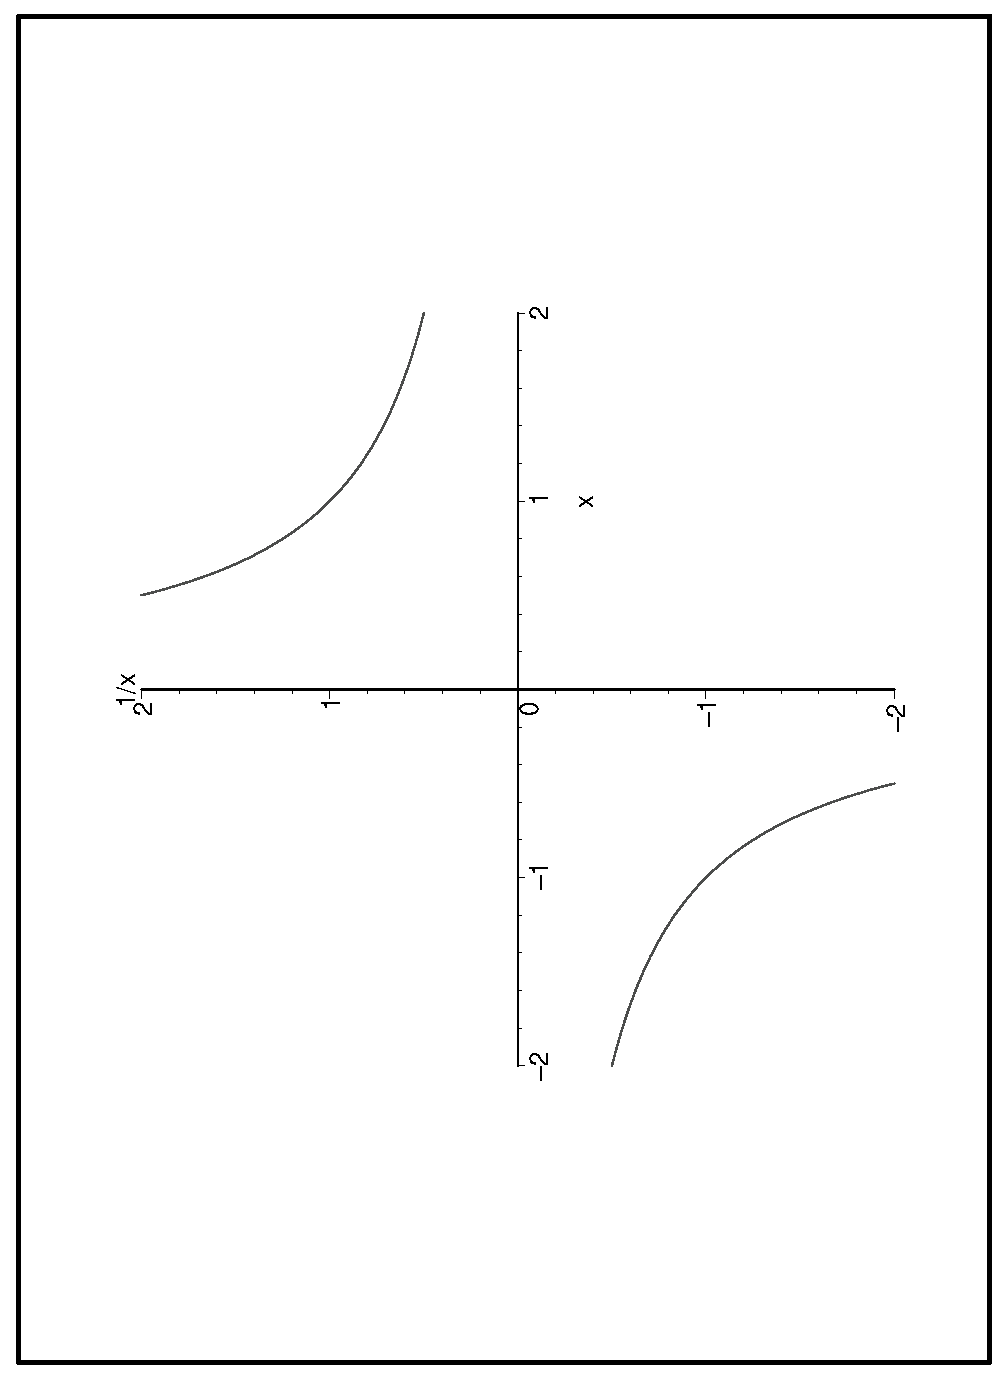
\includegraphics[ angle=270]{grafiekjes/1overx}}
%\end{center}

%\begin{itemize}
%\item $\displaystyle{\lim_{x \to
%0^+}} \frac 1x = + \infty$ \hspace{1cm} en \hspace{1cm}
%$\displaystyle{\lim_{x \to 0^-}} \frac 1x = - \infty$

%Merk op dat $\displaystyle{\lim_{x \to  0}} \frac 1x$ niet bestaat
%omdat de linker- en rechterlimiet verschillend zijn.

%\\
%De rechte $x = 0$ (de y-as) noemen we een \textit{ verticale
%asymptoot} van (de grafiek van) $f$.

%\item $\displaystyle{\lim_{x \rightarrow + \infty} \frac1x = 0}$
%\hspace{1cm} en \hspace{1cm} $\displaystyle{\lim_{x \rightarrow -
%\infty} \frac 1x = 0}$

%De rechte $y=0$ (de x-as) noemen we een \textit{ horizontale
%asymptoot} van (de grafiek van) $f$.
%\item $\displaystyle{\lim_{x \to
%2}} \frac 1x = \frac12$
%\end{itemize}
\subsection*{Rekenregels}
De limiet
van een som is de som van de limieten, de limiet van een product is
het product van de limieten en de limiet van een quoti\"ent is het
quoti\"ent van de limieten, tenzij je daardoor een onbepaalde vorm
krijgt.

{\bf onbepaalde vormen} :
\[\aligned
& (+ \infty) + (-\infty) \\
& (- \infty) + (+ \infty) \\
& 0 \cdot (+ \infty) \quad \text { en } \quad (+ \infty) \cdot 0 \\
& 0 \cdot (- \infty) \quad \text { en } \quad (- \infty) \cdot 0
\\
& \frac{0}{0} \quad \text { en} \quad \frac{\infty}{\infty}
\endaligned
\]
\subsection*{Oefeningen}
\begin{enumerate}
\item Vind de limieten met de hulp van de grafieken van $e^x$ en $\ln x$:
\begin{itemize}

\item $\ds \lim_{x \rightarrow + \infty} e^x = $
\item $\ds \lim_{x \rightarrow - \infty} e^x = $

\item $\displaystyle{\lim_{x \to  0^+}} (e^{\frac 1x}) = $
\item $\displaystyle{\lim_{x  \to  0^-}} (e^{\frac 1x}) = $
\item $\ds \lim_{x \rightarrow + \infty} \ln x = $
\item $\displaystyle{\lim_{x \to  0^+}} \ln x = $
\item $\ds \lim_{x \rightarrow - \infty} \ln x = $
\item $\ds \lim_{x \rightarrow + \infty} \ln(1+ \frac 1x) = $
\end{itemize}

\item Limieten in nulpunt van noemer dat geen nulpunt van teller is:
\begin{enumerate}
\item $\displaystyle{\lim_{x \rightarrow 1}} \frac {1}{(x-1)^2}$
\item $\displaystyle{\lim_{x \to 1^+}} \frac{x^2
+ x - 1}{x-1}$
\item $\displaystyle{\lim_{x \to 1^-}} \frac{x^2
+ x - 1}{x-1}$
\item $\displaystyle{\lim_{x  \to 1^-}} \frac{x
-3} {x^2-1}$
\item $\displaystyle{\lim_{x  \to \pi^-}}\frac{x}{\sin x}$
\end{enumerate}
\item Limieten in nulpunt van teller en noemer:
\begin{enumerate}
\item
$\displaystyle{\lim_{x \to 2}} \frac{x^2 - 4 }{x-2} $
%\item
%$\displaystyle{\lim_{x
% \to 1^-}} \frac{x^3 - 3x +2}{(x-1)^3}$
 \item $ \ds \lim_{x \rightarrow 3} \frac {\sqrt{2x+3}
-3}{x^2-9} $
 \end{enumerate}

\item Limieten in $+ \infty$ en $- \infty$:
\begin{enumerate}
\item $\displaystyle{\lim_{x \rightarrow + \infty}} (2x^3 - 5x^2)$
\item $\displaystyle{\lim_{x \rightarrow - \infty}} \frac{-x^2 + 3x
- 2}{3x-7}$
\item $\displaystyle{\lim_{x \rightarrow - \infty}} (\sqrt{4x^2 + 7x} + 3x)$
\item $\displaystyle{\lim_{x \rightarrow - \infty}} (\sqrt{4x^2 + 7x} + 2x)$
\end{enumerate}


\end{enumerate}
\subsection*{Oplossingen}
\begin{enumerate}
\item zie slides
\item

(a) $+ \infty$, (b) $+ \infty$, (c) $ - \infty$, (d) $ + \infty$,
(e) $ + \infty$

\item

(a) 4, 
%(b) $- \infty$, 
(b) $ \ds \frac{1}{18}$

\item

(a) $+ \infty$, (b) $+ \infty$, (c) $- \infty$,(d)  $\ds - \frac74$


\end{enumerate}
\end{document}
